\chapter{Free Vibrations} \label{ch:free-vibrations}

\section{Overview} \label{ch3:sec-simple-springs}
Any physical system that undergoes SHM is associated with...
\begin{itemize}
	\item a constant representing the \kcol{elasticity} of the system $\longrightarrow$ kinetic energy
	\item a constant representing the \mcol{inertia} of the system $\longrightarrow$ potential energy
\end{itemize}

Consider the motion of a mass $m$ on a spring with spring constant $k$:
\begin{align}
	\text{From Newton's Law: }&
	\mcol{m}\ddot{x} + \kcol{k}x = 0 \label{ch3:eq-NL} \\
	\text{From Conservation of Energy: }&
	\frac{1}{2}\mcol{m}\dot{x}^2 + \frac{1}{2}\kcol{k}x^2 = E \label{ch3:eq-CE}
\end{align}

Any equation matching either of the forms above\footnote{Notice that \eqref{ch3:eq-NL} happens to be the \textit{first derivative} of  \eqref{ch3:eq-CE}.} automatically has as a solution:
\begin{equation}
\boxed{x = A \cos(\omega t+\alpha)\where\omega^2 = \frac{\kcol{k}}{\mcol{m}}} \label{ch3:eq-SHM-soln}
\end{equation}

Some of the \textbf{simple harmonic oscillators} (SHO) in this chapter are analyzed through comparison with \eqref{ch3:eq-NL}, while others, with \eqref{ch3:eq-CE}. Although the systems have differing elastic and inertial constants, they share the following similarities:
\begin{equation}
	\boxed{
		\omega^2 = \frac{\kcol{\text{elasticity}}}{\mcol{\text{inertia}}} \hhtab 
		T = \frac{2\pi}{\omega} \hhtab 
		f = \frac{\omega}{2\pi}}
\end{equation}

\subsection{Effects of gravity}

\begin{figure}
	\centering
	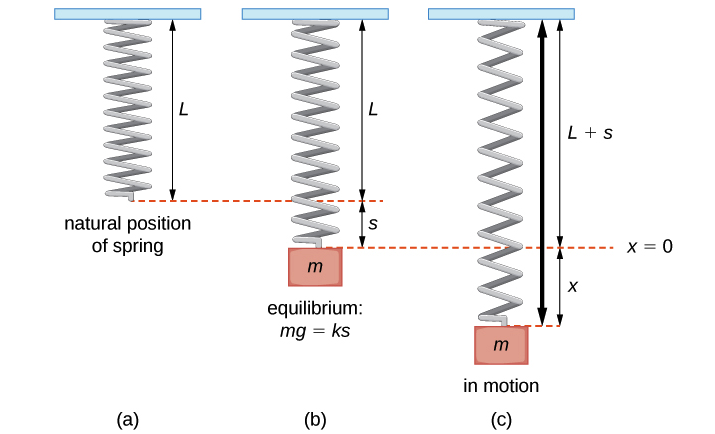
\includegraphics[scale=0.4]{phys232/Ch3-g-new-eqm} \caption{Gravity shifts the equilibrium position of a SHO by a distance $h=mg/k$.}\label{ch3:fig-g-new-eqm-pos}
\end{figure}

Gravity only changes the equilibrium position of a SHO, without changing the amplitude, period, or frequency:
\begin{align*}
	m\ddot{x} &= -kx + mg \\
	& = -k(x - \frac{mg}{k}) \\
	& = -k(x - h) \where h=\frac{mg}{k}
\end{align*}
Let $y=x-h$. This implies $\ddot{y} = \ddot{x}$. Therefore,
\begin{align*}
	&m\ddot{y} = -ky \\
	&m\ddot{y} + ky = 0 
\end{align*}
i.e. we still have SHM!

We can interpret $h$ as the initial change in position that occurs when the mass is hung or the floating object is placed in a liquid, and we wait for the system to reach \emph{static equilibrium} (see Figure~\ref{ch3:fig-g-new-eqm-pos}).
\[ mg = kh \Longrightarrow \boxed{h = \frac{mg}{k}} \]


\subsection{Overview of the systems analyzed}

\begin{fullwidth}
\centering
\renewcommand{\arraystretch}{2.5}
\begin{tabular}{lll}
	\hline
	Type of system & Equation & $\omega^2$ \\ \hline
	Mass on spring &
		$\mcol{m}\ddot{x} + \kcol{k}x = 0$ &
		$\dfrac{\kcol{k}}{\mcol{m}}$
		\\
	\parbox{4cm}{\hyperref[ch3:sec-wire]{Mass on wire} \\\footnotesize{(with Young's Modulus $Y$)}} &
		$\mcol{m}\ddot{x} + \kcol{\frac{AY}{l_0}}x = 0$ &
		$\dfrac{\kcol{AY}}{\kcol{l_0}\mcol{m}} = \dfrac{g}{h}$ 
		\\
	\hyperref[ch3:sec-floating]{Floating objects} &
		$\mcol{m}\ddot{y} + \kcol{g\rho A}y = 0$ &
		$\dfrac{\kcol{g\rho A}}{\mcol{m}} = \dfrac{g}{h}$ 
		\\
	\hyperref[ch3:sec-torsional]{Torsional oscillations} &
		$\mcol{I}\ddot{\theta} + \kcol{c}\theta = 0$ &
		$\dfrac{\kcol{c}}{\mcol{I}}$ 
		\\
	\parbox{3.5cm}{\hyperref[ch3:sec-air]{Spring of air} \\\footnotesize{(isothermal conditions)}} &
		$\mcol{m}\ddot{y} + \kcol{\frac{Ap}{l}}y = 0$ &
		$\dfrac{\kcol{Ap}}{\kcol{l}\mcol{m}}$ 
		\\
	\parbox{3.5cm}{\hyperref[ch3:sec-air]{Spring of air} \\\footnotesize{(adiabatic conditions)}} &
		$\mcol{m}\ddot{y} + \kcol{\frac{A\gamma p}{l}}y = 0$ &
		$\dfrac{\kcol{A\gamma p}}{\kcol{l}\mcol{m}}$ 
		\\
	\hline
		Mass on spring &
			$\frac{1}{2}\mcol{m}\dot{x}^2 + \frac{1}{2}\kcol{k}x^2 = E $ &
			$\dfrac{\kcol{k}}{\mcol{m}}$
			\\
		\hyperref[ch3:sec-simple-pendulum]{Simple pendulum} &
			$\frac{1}{2}\mcol{I}\dot{\theta}^2 + \frac{1}{2}\kcol{mgl}\theta^2 = E $ &
			$\dfrac{\kcol{mgl}}{\mcol{I}} = \dfrac{\kcol{mgl}}{\mcol{ml^2}}= \dfrac{\kcol{g}}{\mcol{l}}$ 
			\\
		\parbox{5cm}{\hyperref[ch3:sec-complex-pendulum]{Arbitrary pendulum} \footnotesize(with radius of gyration $k$, centre of mass at distance $h$ from point of suspension)}&
			$\frac{1}{2}\mcol{m(k^2+h^2)}\dot{\theta}^2 + \frac{1}{2}\kcol{mgh}\theta^2 = E $ &
			$\dfrac{\kcol{gh}}{\mcol{k^2+h^2}}$ 
			\\
		\hyperref[ch3:sec-uTube]{Water in a U-tube} &
			$\frac{1}{2}\mcol{\rho Al}\dot{y} + \frac{1}{2}\kcol{(2g\rho A)}y^2 = E$ &
			$\dfrac{\kcol{2g}}{\mcol{l}}$ 
			\\
		\hyperref[ch3:sec-torsional]{Torsional oscillations} &
			$\frac{1}{2}\mcol{I}\dot{\theta} + \frac{1}{2}\kcol{c}\theta^2 = E$ &
			$\dfrac{\kcol{c}}{\mcol{I}}$ 
			\\
		\parbox{5cm}{	\hyperref[ch3:sec-massive-springs]{Massive springs} \\\footnotesize{(with mass $M$)}} &
			$\frac{1}{2}\mcol{\left(m + \frac{1}{3}M \right)}\dot{x} + \frac{1}{2}\kcol{k}x^2 = E$ &
			$\dfrac{\kcol{k}}{\mcol{m + M/3}}$ 
			\\
		\hline
	\end{tabular}
	\renewcommand{\arraystretch}{1}
\end{fullwidth}


\section{Solving for the equation of motion of a harmonic oscillator}

\begin{proof}[Solving for the equation of motion]
Rewrite \eqref{ch3:eq-NL} in terms of $k/m$:
\begin{align}
m\ddot{x} + kx &= 0 \notag\\
\ddot{x} + \frac{k}{m}x &= 0 \notag\\
\ddot{x} + \omega^2 x  &= 0 \label{ch3:eq-xdd}
\end{align}

\eqref{ch3:eq-xdd} implies $\ddot{x}$ is a multiple of $x$. This is a property of the exponential function, so write: 
\begin{equation}
	x=Ce^{pt} \label{ch3:eq-xCPT}
\end{equation}
where $p$ is a dimensional constant such that $pt$ is dimensionless, and $C$ is a coefficient.
%
\begin{align*}
\intertext{Sub \eqref{ch3:eq-xCPT} back into \eqref{ch3:eq-xdd}:}
\frac{d^2}{dt^2}(Ce^{pt})+\omega^2(Ce^{pt}) &= 0\\
p^2Ce^{pt}+\omega^2Ce^{pt}&=0 \\
Ce^{pt}(p^2+\omega^2) &=0 \\
\Longrightarrow p^2 + \omega^2 &= 0 \\
p^2 &= -\omega^2 \\
p &= \pm j\omega
\end{align*}

Because we have two possibilities for $p$, we can write a more-general solution for \eqref{ch3:eq-xdd}%
\footnote{In general, when working with second-order differential equations like \eqref{ch3:eq-xdd}, we need to introduce two constants -- one for each level of integration. These constants could be $C_1, C_2$, or as we will see, $A$ and $\alpha$.}:
\begin{equation}
	 x = C_1e^{j\omega t}+C_2e^{-j\omega t}	\label{ch3:eq-complex-general-sol}
\end{equation}

Geometrically, $x$ is the sum of two vectors: one with length $C_1$ rotating CCW and another with length $C_2$ going CW, both with the same angular displacement $\omega t$ (see Figure~\ref{ch3:fig-complex-sols}a).

In order to produce a harmonic oscillation along the $x$-axis, the $y$-components of the vectors must cancel. This is also the case when we have an initial phase angle $\alpha\neq 0$ (see Figure~\ref{ch3:fig-complex-sols}b).

\begin{figure}
	\centering
	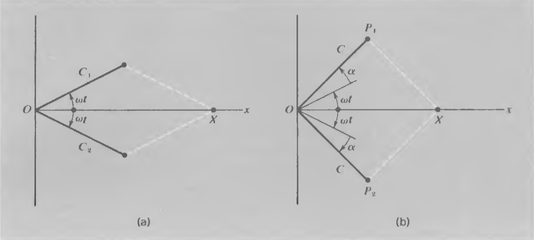
\includegraphics[scale=0.5]{phys232/Ch3-adding-complex-solutions.png} \caption{Superposition of complex solutions of \eqref{ch3:eq-xdd} with (a) $\alpha=0$ and (b) $\alpha\neq 0$. For the length $OX$ to represent a harmonic oscillation, $C1=C2$.}
	\label{ch3:fig-complex-sols}
\end{figure}


For the $y$-components to cancel, we need $C_1=C_2$. Hence\footnote{Reminder: $\cos(-\theta)=\cos\theta$ and $\sin(-\theta)=-\sin\theta$}, using Euler's identity \eqref{ch1:eq-eulers-identity},
\begin{align*}
x
&=Ce^{j(\omega t +\alpha)} + Ce^{-j(\omega t +\alpha)} \\
&=C[\cos(\omega t + \alpha) + j\sin(\omega t + \alpha) \\
&\hhtab\hhtab + \cos(-(\omega t + \alpha)) + j\sin(-(\omega t + \alpha))] \\
&=C[\cos(\omega t + \alpha) + \cancel{j\sin(\omega t + \alpha)} \\
& \hhtab\hhtab + \cos(\omega t + \alpha) - \cancel{j\sin(\omega t + \alpha)}] \\
&= 2C\cos(\omega t + \alpha) \\
\therefore
x &= Acos(\omega t + \alpha) \where A=2C
\end{align*}

This is why, for SHM in general, we can assume solutions of the type:
\begin{equation}
	x=\Re(z) \where z=Acos(\omega t + \alpha)
\end{equation}
\end{proof}


\section{Elastic Wire \& Young's Modulus} \label{ch3:sec-wire}

Apply a force $F_\text{app}$ to one end (e.g., by hanging a mass off it) and let the other end remain fixed. When the wire/rod is in \textit{static equilibrium}, let us define two quantities:

\[ \text{stress} = \frac{F_\text{app}}{A} \where\text{$A$ is the cross-sectional area} \]

\[  \text{strain} = \frac{x}{l_0} \where\text{$x$ is the extension of the wire}  \]

The ratio between these two quantities is a constant $Y$, which we call \textbf{Young's modulus of elasticity} for the material\footnote{... as long as the strain is small enough, such that the material is not permanently deformed when stretched.}:
\begin{equation}
	\boxed{ Y = \frac{\text{stress}}{\text{strain}} = \text{const}} \label{ch3:eq-Youngs-Modulus}
\end{equation}

Let us consider the force $F = -F_\text{app}$ exerted \emph{by} the rod \emph{on} another object. Hence,
\begin{align}
	& Y = \frac{-F/A}{x/l_0} \notag \\
	& \boxed{F = \kcol{\frac{-AY}{l_0}} x } \label{ch3:eq-Youngs-F}
\end{align}


Once a mass $m$ is hung on one end:
\[ \omega^2 = \sqrt{\frac{\kcol AY}{\mcol m \kcol{l_0}}} \]

We can rewrite this in terms of properties more easily measured at static equilibrium, such as $h$, the increase of length reached at static equilibrium after the mass is attached.
\[ \mcol{m}g=\kcol{\frac{AY}{l_0}} h \Longrightarrow \frac{ml_0}{AY}=\frac{h}{g} \]
\begin{equation}
\therefore \omega^2 = \frac{g}{h}  \label{ch3:eq-elastic-wire-result}
\end{equation} 

Remark: this result is similar to that for a simple pendulum (Equation~\ref{ch3:eq-simple-pendulum-result}).

\section{Floating Objects} \label{ch3:sec-floating}

\begin{marginfigure}
	\centering
	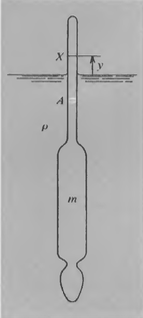
\includegraphics[scale=0.6]{phys232/Ch3-floating.png}
	\caption{Floating object at a vertical displacement of $y$ from its equilibrium position.}
	\label{ch3:fig-floating}
\end{marginfigure}

Let the floating object (of mass $m$) have a constant cross-sectional area $A$ parallel to the liquid surface.

Recall:
\[ F_\text{buoyancy} = \text{weight of liquid displaced by the floating object} \]
\[ \boxed{F_b  = \kcol{g\rho A}y} \]

where...
\begin{itemize}
	\item $\rho$: density of the liquid
	\item $y$: vertical displacement of the object above equilibrium position
\end{itemize}


By Newton's Law:
\[ \mcol{m}\frac{d^2y}{dt^2} = -\kcol{g\rho A}y \]
\[ \therefore \omega^2 = \frac{\kcol{g\rho A}}{\mcol{m}} \]

We can, again, rewrite $\omega^2$ in terms of $h$, the change in equilibrium position when the object is placed in the liquid and reaches static eqm:
\[ \mcol{m}\cancel{g}=\kcol{\cancel{g}\rho A} h
\Longrightarrow
h = \frac{m}{\rho A} \]
\[ \therefore \omega^2 = \frac{g}{h} \]


This is analogous to the $\omega^2$ of an elastic wire, seen earlier in \eqref{ch3:eq-elastic-wire-result}. 


\section{The Pendulum}
\begin{figure}
	\centering
	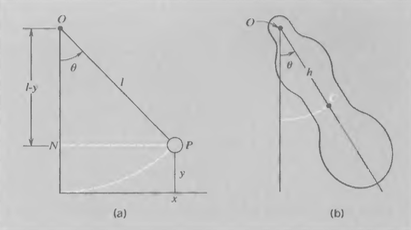
\includegraphics[scale=0.6]{phys232/Ch3-pendulum.png} \caption{(a) Simple pendulum; (b) pendulum of arbitrary shape with its centre of mass at $C$.}\label{ch3:fig-pendulum}
\end{figure}

Let $\theta$ represent the angular displacement of the pendulum. Assume small $\theta$ such that $y \ll x$. 


\subsection{Simple Pendulum} \label{ch3:sec-simple-pendulum}
By the Pythagorean Theorem (see Figure~\ref{ch3:fig-pendulum}):
\begin{align}
l^2 &= x^2 + (l-y)^2  \notag \\	
\cancel{l^2} &= x^2 + \cancel{l^2} - 2ly + y^2 \notag \\
x^2 &= 2ly - {y^2} \notag \\
x^2 &\approx 2ly  \notag \\
\Longrightarrow y &\approx \frac{x^2}{2l} \label{ch3:eq-pendulum-pythag}
\end{align}

In addition,
\begin{equation}
v^2=\left( \frac{dx}{dt} \right)^2 + \left(\frac{dy}{dt} \right)^2
\approx  \left( \frac{dx}{dt} \right)^2 \label{ch3:eq-pendulum-v2}
\end{equation}

By the Conservation of Energy and using the approximations \eqref{ch3:eq-pendulum-pythag} and  \eqref{ch3:eq-pendulum-v2}:
\begin{align}
\frac{1}{2} mv^2 + mgy &= E \notag \\
\frac{1}{2} \mcol{m} \left( \frac{dx}{dt} \right)^2 + \frac{1}{2} \kcol{\frac{mg}{l}} x^2 &= E  \label{ch3:eq-pendulum-E}
\end{align}


We can rewrite this result in terms of $\theta$ by substituting in\footnote{Use the small angle approximation $\cos\theta \approx 1-\frac{\theta^2}{2}$, from Equation~\eqref{ch1:eq-small-angle-cos}}:
\begin{equation*}
v = l\left(\frac{d\theta}{dt}\right) \andd
y = l(1-\cos\theta) \approx \frac{1}{2}l\theta ^2
\end{equation*}

So, \eqref{ch3:eq-pendulum-E} becomes:
\begin{equation}
	\frac{1}{2} \mcol{ml^2} \left( \frac{d\theta}{dt} \right)^2 + \frac{1}{2} \kcol{mgl} \theta^2 = E \label{ch3:eq-pendulum-E-theta}
\end{equation}

Both \eqref{ch3:eq-pendulum-E} and \eqref{ch3:eq-pendulum-E-theta} imply that:
\begin{equation}
	\therefore \omega^2 = \frac{g}{l} \label{ch3:eq-simple-pendulum-result}
\end{equation}


\subsection{Pendulum of an Arbitrary Shape} \label{ch3:sec-complex-pendulum}
Consider a pendulum of arbitrary shape suspended at point $O$, with center of mass $C$. Suppose these points are separated by a distance $h$, as shown in Figure~\ref{ch3:fig-pendulum}b.

Let $I_O$ represent the moment of inertia \emph{about an axis passing through $O$}. Then:
\begin{equation*}
KE = \frac{1}{2} \mcol{I_O}\left( \frac{d\theta}{dt} \right)^2 \andd
PE = \frac{1}{2} \kcol{mgh}\theta^2 
\end{equation*}
Note that $PE_\text{pendulum} = PE_\text{centre of mass}$. The above assumes $PE = 0$ at the lowest height reached by the CM.
\begin{equation} 
	\Longrightarrow
	\frac{1}{2} \mcol{I_O}\left( \frac{d\theta}{dt} \right)^2 + \frac{1}{2} \kcol{mgh}\theta^2 = E \label{ch3:eq-pendulumEO}
\end{equation}

\paragraph{Re-expressing the result in terms of $I_\text{CM}$}
From the \emph{parallel axis theorem}: recalling that the distance $OC$ is $h$, we have:
\begin{align*}
	I_O &= I_\text{CM} + mh^2 \\
	&= mk^2 + mh^2
\end{align*}

where $k$ is the \emph{radius of gyration}\footnote{The radius of gyration $k$ is the length of a simple pendulum (consisting of a point mass and a light cord) that could ``replace" the complex pendulum while still keeping the same mass $m$.}. Thus,
\begin{align*}
	KE_C %&= \frac{1}{2} ( I_\text{CM} + mh^2 ) \left( \frac{d\theta}{dt} \right)^2 \\
	&= \frac{1}{2} m(k^2 + h^2 ) \left( \frac{d\theta}{dt} \right)^2
\end{align*}

Then, \eqref{ch3:eq-pendulumEO} becomes:
\[ \frac{1}{2} \mcol{m(k^2+h^2)} \left( \frac{d\theta}{dt} \right)^2  + \frac{1}{2} \kcol{mgh}\theta^2 = E \]

\begin{equation*}
	\therefore \omega^2 = \frac{\kcol{gh}}{\mcol{m(k^2+h^2)}}
\end{equation*}

This result is analogous to what we found for an elastic wire (Equation~\ref{ch3:eq-elastic-wire-result}).

\section{Liquid in a U-Tube} \label{ch3:sec-uTube}

\begin{figure}
	\centering
	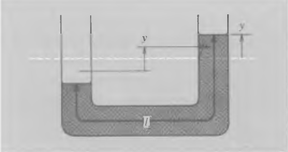
\includegraphics[scale=0.8]{phys232/Ch3-utube.png}
	\caption{Oscillating liquid column in a U-tube.}
	\label{ch3:fig-utube}
\end{figure}

Examine the vertical displacement $y$ of the liquid surface from equilibrium in a U-tube with uniform cross-sectional area $A$.

Define $l$, the total length of the liquid column, and $\rho$, the liquid's density.

When liquid \textit{rises} a height of $y$ in one end, the liquid in the other end \textit{sinks} by the same height $y$. The mass%
\footnote{Recall that density = mass/volume, so $m=\rho V=\rho Ay$.}
of the liquid that moves is $\rho Ay$. 

Assume the whole liquid, which has mass $\rho Al$, moves with speed $dy/dt$. So,
\[ KE = \frac{1}{2} \rho Al \left(\frac{dy}{dx}\right)^2 \andd
PE = g\rho Ay^2 \]
\[ \Longrightarrow \frac{1}{2} \mcol{\rho Al} \left( \frac{dy}{dt} \right)^2 
+ \frac{1}{2} \kcol{(2g\rho A)} y^2 = E  \] 

\begin{equation}
\therefore \omega^2 = \frac{\kcol{2g}}{\mcol{l}} \label{ch3:eq-utube-result}
\end{equation}

Again, the result for a U-tube \eqref{ch3:eq-utube-result} is comparable to that for an elastic wire \eqref{ch3:eq-elastic-wire-result}.

\section{Torsional Oscillations} \label{ch3:sec-torsional}

If the torque $\tau \propto$ angular displacement $\theta$ between two ends of an object,
\[ \tau=-\kcol{c}\theta \where\text{$c$ is the torsion constant of the system.} \]

Stored potential energy: \[ U= -\int \tau d\theta = \frac{1}{2} \kcol{c}\theta^2 \]

If one end has a moment of inertia $\mcol{I}$ and the inertia of the twisted system itself is negligible, then by the conservation of energy:
\[ \frac{1}{2} \mcol{I} \left( \frac{d\theta}{dt}\right)^2 + \frac{1}{2} \kcol{c}\theta^2 = E \]

Thus:
\begin{equation*}
\omega^2 = \frac{\kcol{c}}{\mcol{I}}
\end{equation*}


\subsection{Shear Modulus}

\begin{figure}
	\centering
	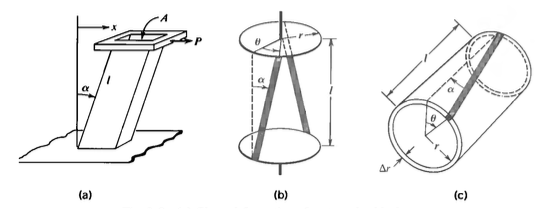
\includegraphics[scale=0.55]{phys232/Ch3-shear-torsion.png}
	\caption{(a) Shear deformation of a rectantular block; (b) Torque on rectangular strips during shear deformation; (c) A twisted tube can be considered as a collection of strips undergoing shear.}
	\label{ch3:fig-shear-torsion}
\end{figure}

When we apply a horizontal force $F_\text{app}$ to the board in Figure~\ref{ch3:fig-shear-torsion}a, two of the sides change from rectangles to parallelograms. This is called a \textbf{shear deformation}.

Define an \textbf{angle of shear, $\alpha$}:
\[ \alpha = \frac{x}{l} \]

It turns out that, just like when we stretch an elastic wire (Section~\ref{ch3:sec-wire}), the ratio between stress and the ``angular strain" is a constant.

We call this the \textbf{shear modulus} or \textbf{modulus of rigidity} $n$ for the material (cf. Equation~\ref{ch3:eq-Youngs-Modulus}):
\[  n= \frac{F_\text{app}/A}{\alpha} = \text{const} \]

Let us consider the force $F=-F_\text{app}$ exerted \emph{by} the sheared material \emph{onto} the board. Hence,
\[  n = \frac{-F/A}{x/l} \]
\begin{equation}
	\boxed{F = \kcol{\frac{-nA}{l}} x}  \label{ch3:eq-torsional-F}
\end{equation}

Notice that \eqref{ch3:eq-torsional-F} for {shear deformations} is comparable to \eqref{ch3:eq-Youngs-F} for {longitudinal deformations}\footnote{Another modulus also exists: the \textbf{bulk modulus}, $K$, which describes the resistance of a material to changes in volume -- more about this in Section~\ref{ch3:sec-bulk-modulus}.}.

\subsection{Torque due to shear}
Refer to Figure~\ref{ch3:fig-shear-torsion}b, where two disks of radius $r$ on spindles are connected by two rectangular strips of material, each with cross-sectional area $A$.

Twist one spindle through a small $\theta$; the end of each strip undergoes shear through a distance $x=r\theta$. 

Substituting this into \eqref{ch3:eq-torsional-F}, we see that the restoring force $\Delta F$ exerted by each strip tangentially to the disk is:
\[ \Delta F = -\kcol{nA\frac{r}{l}} \theta \]

Hence, there is a restoring torque exerted by \emph{each} strip about the axis of twist:
\begin{align*}
	\Delta\tau &= r\,dF  \notag \\
	&= -\frac{nAr^2\theta}{l} 
\end{align*}

\paragraph{Thin-Walled Tube}
Refer to Figure~\ref{ch3:fig-shear-torsion}c, where we will consider a twisted, thin-walled tube as a collection of many strips, each undergoing shear and contributing restoring torques about the axis of twist.

Let the radius be $r$ and the wall thickness be $\Delta r$. This means the cross-sectional area is $A=2\pi r \Delta r$. The restoring torque from a \emph{thin ring of strips} is thus:
\begin{equation}
\Delta \tau = -\frac{2\pi nr^3\Delta r}{l} \theta  \label{ch3:eq-thinTube_dtau}
\end{equation}

\paragraph{Solid Tube}
We can model a \textit{solid} tube or cylinder as multiple thin-walled tubes. Integrate \eqref{ch3:eq-thinTube_dtau} to obtain, as a total restoring torque:
\begin{equation*}
	\boxed{\tau = -\kcol{\frac{\pi nr^4}{2l}} \theta}
\end{equation*}

\section{``The Spring of Air"} \label{ch3:sec-air}

\begin{marginfigure}
	\centering
	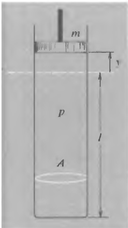
\includegraphics[scale=0.8]{phys232/Ch3-air.png}
	\caption{Piston in a vertical air column.}
	\label{ch3:fig-air}
\end{marginfigure}

Consider a closed piston-gas system, as pictured in Figure~\ref{ch3:fig-air}.

Let $m$ represent the mass of the movable piston, and $p$, the pressure of the gas inside the tube.

When the piston moves a distance of $y$ from equilibrium position $l$, the pressure of the gas changes by $\Delta p$.

\subsection{Isothermal conditions}
Under {isothermal} (constant temperature) conditions, \emph{Boyle's Law} applies\footnote{Recall also the product rule for differentiation}:
\begin{align*}
pV &= \text{const} \\
p\Delta V + V\Delta p &= 0
\end{align*}

But... the equilibrium volume was $V = Al$ and the change in volume is $\Delta V = Ay$.
\[ p(Ay) + (Al)\Delta p = 0 \]
\[ \Delta p = -\frac{py}{l} \]

Because $F=PA$:
\begin{equation}
	\boxed{F=-\kcol{\frac{Ap}{l}} y } \label{ch3:eq-pistonF}
\end{equation}

\subsection{Bulk Modulus} \label{ch3:sec-bulk-modulus}

Compare \eqref{ch3:eq-pistonF} with \eqref{ch3:eq-Youngs-F} for stretching a rod. Here, $p$ plays a role analogous to $Y$. We can call $p$ the \textbf{isothermal bulk modulus} of the gas:
\begin{equation*}
	K_\text{isothermal} = p
\end{equation*}

More formally, the \textbf{bulk modulus} of a specimen is defined as:
\begin{align*}
	K &= -\frac{dp}{dV/V} \notag \\
	\Aboxed{K &= -V\frac{dp}{dV}}
\end{align*}

\subsection{Adiabatic conditions}

In general, $K_\text{isothermal}$ is not a good descriptor of the elasticity of an air column.
\begin{itemize}
	\item When a gas is compressed, it becomes \emph{warmer} because of the work being done on it.
	\item Heating results in a greater restoring force.
	\item We expect a higher value than $p$ for the elasticity of the gas.
\end{itemize}

In \textbf{adiabatic conditions} (closed system; no flow of heat in/out of the gas), we have:
\begin{align*}
pV^\gamma &= \text{constant} \\
\Longrightarrow \ln p + \gamma\ln V &= \text{const} \tag{taking $\ln$ of both sides} \\
\Longrightarrow \frac{1}{p}\frac{dp}{dV} + \frac{\gamma}{V} &= 0 \tag{integrating both sides} 
\intertext{By the definition of $K_\text{adiabatic}$,}
K_\text{adiabatic} &= -V \frac{dp}{dV} \\
\Aboxed{K_\text{adiabatic} &= \gamma p}
\end{align*}

Because elasticity is enhanced under adiabatic conditions, and the frequency of vibrations is increased too:
\begin{equation*}
	\therefore
	\omega^2_\text{isothermal} \propto \kcol{p} \andd
	\omega^2_\text{adiabatic} \propto \kcol{\gamma p}
\end{equation*}

\section{Massive Springs} \label{ch3:sec-massive-springs}

\begin{figure}
	\centering
	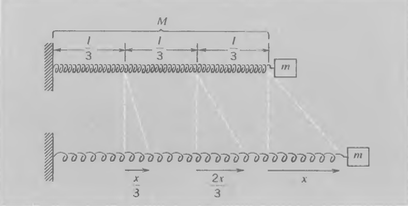
\includegraphics[scale=0.75]{phys232/Ch3-massive-spring.png} \caption{Uniform extension of a massive spring with mass $M$.}\label{ch3:fig-massive-spring}
\end{figure}

Suppose this time the spring itself has a mass of $M$. Suppose that it has a spring contant $k$ and that there is a mass $m$ attached to it. Let the equilibrium length of the spring be $l$.

The \emph{linear mass density} of the spring is $ \lambda = {M}/{l} $.

Consider an infinitesimal segment of the spring initially at a distance $s$ from the fixed end $(0 \leq s \leq l)$, with a width $ds$. Its mass is:
\[ dM = \lambda\,ds = \frac{M}{l}\,ds \] 

\paragraph{Assumption} Each point on the spring undergoes a displacement proportional to its distance from the fixed end (Figure~\ref{ch3:fig-massive-spring}). So, the displacement and speed of the segment are:
\[ \text{displacement} = \frac{s}{l} \, x \andd
\text{speed} = \frac{s}{l} \frac{dx}{dt} 
\]

Its kinetic energy is \[ dK = \frac{1}{2}\left( \frac{M}{l} ds \right) \left( \frac{s}{l} \frac{dx}{dt} \right)^2 = \frac{M}{2l^3} \left( \frac{dx}{dt} \right)^2 s^2 \, ds \]

For the kinetic energy of the whole spring, integrate, treating $dx/dt$ as a constant:
\begin{align*}
K_\text{spring} &= \frac{M}{2l^3} \left( \frac{dx}{dt} \right)^2  \int_0^{l} s^2 \, ds \\
&= \frac{1}{6}M\left(\frac{dx}{dt}\right)^2
\end{align*}

So, the energy-conservation statement for the whole system becomes:
\begin{align*}
\frac{1}{2}m\left(\frac{dx}{dt}\right)^2 + \frac{1}{6}M\left( \frac{dx}{dt}\right)^2 + \frac{1}{2}kx^2 &= E  \\
\frac{1}{2} \mcol{\left( m + \frac{M}{3} \right)} \left(\frac{dx}{dt}\right)^2 + \frac{1}{2} \kcol{k} x^2 &= E
\end{align*}
\[ \therefore \omega^2 = \frac{\kcol{k}}{\mcol{m+M/3}} \]

This is the equivalent of taking a massless spring (see Equation~\ref{ch3:eq-SHM-soln}), and then adding a mass of $m + M/3$ to the end.

In reality, our model holds only when $M \ll m$. Otherwise, the force along the spring is not constant -- we can no longer assume that the elongation of a point is proportional to its distance from the fixed end.

\section{Decay (Damping) of Free Oscillations}

In general, resistive forces act in a direction opposite to $\vec{v}$ and have magnitude:
\[ F_b = b_1v + b_2v^2\]

When $v$ is small in comparison to $b_1/b_2$, we can make an approximation:
\begin{equation*}
	\boxed{\vec{F}_b = -b\vec{v}}
\end{equation*}

If our mass-spring system (cf. Section~\ref{ch3:sec-simple-springs}) had damping, our statement of Newton's Law would have been:
\begin{align}
	m\ddot{x} &= -kx - bv \notag \\
	m\ddot{x} + b\dot{v} + kx &= 0 \notag  \\
	\Aboxed{\ddot{x} + \gamma \dot{x} + \omega_0^2 x &= 0} \label{ch3:eq-damping-NL}
\end{align}
where
\[ \boxed{\gamma = \frac{b}{m} \andd \omega_0 = \frac{k}{m}} \]

Interpretation:
\begin{itemize}
	\item $\gamma$: damping constant (with dimensions of frequency)
	\begin{itemize}
		\item We will also that see it represents the reciprocal of the time required for the energy to decrease to $1/e$ of its initial value (Section~\ref{ch3:sec-quality-factor})
	\end{itemize}
	\item $\omega_0$: angular frequency of the system if \emph{damping were absent}
\end{itemize}

The solution to \eqref{ch3:eq-damping-NL} when there is \textbf{underdamping} $(\omega_0>\gamma/2)$ is:
\begin{equation}
\boxed{
	 x = A_0 e^{-\gamma t/2} \cos(\omega t + \alpha) \where \omega ^2 = \omega_0^2 - \frac{\gamma^2}{4} 
}	\label{ch3:eq-damping-solution}
\end{equation}

We can interpret $\omega$ as the angular frequency of the \emph{damped oscillator}.


\subsection{Underdamping $(\omega_0 > \gamma/2)$}
\begin{proof}[Solving for the equation of motion]
Assume $x$ is the real part of a rotating vector $z$. So:
\begin{equation*}
	\ddot{z} + \gamma \dot{z} + \omega_0^2 z = 0
\end{equation*}

Assume the following solution\footnote{Note that this assumed solution contains two constants -- this takes into account that \eqref{ch3:eq-damping-NL} is a second-order differential equation.}:
\begin{equation}
z=A_0 e^{j(pt+\alpha)} \label{ch3:eq-damping-assumed-z}
\end{equation}

Substitute to obtain:
\begin{align}
	(A_0 j^2 p^2 e^{j(pt+\alpha)}) + \gamma (A_0 jpe^{j(pt+\alpha)}) + \omega_0^2 (A_0 e^{j(pt+\alpha)}) &= 0 \notag \\
	A_0 e^{j(pt+\alpha)}(-p^2 + jp \gamma + \omega_0^2) &= 0 \notag \\
	\Longrightarrow (-p^2 + jp \gamma + \omega_0^2) &= 0 \label{ch3:eq-damping-pj}
\end{align}

$p$ cannot be a purely real number -- if that were the case, $jp\gamma$ would not get cancelled. So, assume:
\begin{equation} 
	p = n + js \where \text{$n,s$ are real} \label{ch3:eq-damping-p}
\end{equation}
\[ \Longrightarrow p^2 = n^2 + 2jns - s^2 \]

Substitute into \eqref{ch3:eq-damping-pj}:
\begin{align}
	 (-(n^2 + 2jns - s^2) + j \gamma (n+js) + \omega_0^2) &= 0 \notag \\
	-n^2 - 2jns + s^2 + nj \gamma - s \gamma + \omega_0^2 &= 0 \notag \\
	\underbrace{(-n^2 + s^2  - s \gamma + \omega_0^2)}_\text{real part} +  \underbrace{j(-2ns + n \gamma)}_\text{imaginary part} &= 0 \label{ch3:eq-damping-real-imag}
\end{align}

Both the real and the imaginary parts of \eqref{ch3:eq-damping-real-imag} must equal zero:
\begin{align*}
	\text{Real part: } \htab & -n^2 + s^2  - s \gamma + \omega_0^2 = 0 \\
	\text{Imaginary part: } \htab &-2ns + n \gamma = 0 
\end{align*}

From the imaginary part,
\[ s=\frac{\gamma}{2}\]
Substitute this into the real part to obtain:
\[ n^2 = \omega_0^2 - \frac{\gamma^2}{4} \]

Returning to our assumed solution for $z$ \eqref{ch3:eq-damping-assumed-z}, substitute in our expressions for $s$ and $n$:
\begin{align*}
	z&=A_0 e^{j((n+js)t+\alpha)}  \\
	z &= A_0 e^{-st} e^{j(nt+\alpha)} \\
	z &= A_0 e^{-st} [ \cos(nt+\alpha) + j\sin(nt+\alpha)  ]
\end{align*}
\[ 	\Longrightarrow x = \Re(z) = A_0 e^{-st}\cos(nt+\alpha) \]
\[ \therefore 
x = A_0 e^{-\gamma t/2} \cos(\omega t+\alpha) \where \omega^2 = \omega_0^2 - \frac{\gamma^2}{4} \]
\end{proof}


\begin{figure}
	\centering
	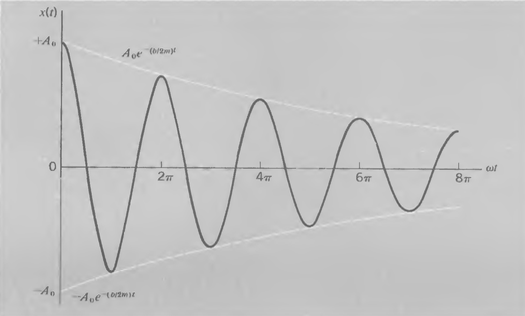
\includegraphics[scale=0.55]{phys232/Ch3-underdamping.png} \caption{Rapidly underdamped harmonic oscillations.}\label{ch3:fig-underdamping}
\end{figure}

Our solution \eqref{ch3:eq-damping-solution} is plotted in Figure~\ref{ch3:fig-underdamping}. Notice that:
\begin{itemize}
	\item A half-period $(\Delta t = \pi/2)$ elapses between zeroes, as well as between successive maxima and minima.
	\item However, the extrema are now only \emph{approximately halfway} between the zeroes.
\end{itemize}

\paragraph{Very Small Damping $(\gamma \ll \omega)$}

When the damping is very small, the motion approximates to SHM at a constant amplitude over a number of cycles around time $t$.

Amplitude around time $t$:
\[ A(t) = A_0 e^{-\gamma t/2} \]

Total energy around time $t$:
\begin{align*}
E(t) = \frac{1}{2}kA^2 
	&= \frac{1}{2}kA_0^2 e^{-\gamma t} \\
\Aboxed{\therefore E(t) &= E_0 e^{-\gamma t} }
\end{align*}
i.e. the total energy decays exponentially.

\paragraph{Quality Factor} \label{ch3:sec-quality-factor}
We can also interpret $\gamma$ as representing the reciprocal of the time required for the energy to decrease to $1/e$ of its initial value. Let us examine why.

We can define a \textbf{quality value} to describe the amount of damping:
\begin{equation}
	\boxed{Q = \frac{\omega_0}{\gamma}} 
	\Longrightarrow 
	\gamma = \frac{\omega_0}{Q}
	\label{ch3:eq-Q-def}
\end{equation}

We can rewrite \eqref{ch3:eq-damping-solution} in terms of $Q$:
\begin{equation}
	\omega^2 = \omega_0^2 \left(1- \frac{1}{4Q^2}\right) \label{ch3:eq-damping-sol-with-Q}
\end{equation}

\eqref{ch3:eq-damping-sol-with-Q} implies that for large $Q$ (i.e. as $Q \to \infty$), $\omega \to \omega_0$. 
Combining \eqref{ch3:eq-Q-def} with \eqref{ch3:eq-damping-solution} gives:
\[ x = A_o e^{-\omega_0 t/2Q} \cos(\omega_0 t + \alpha) \]
\[ \Longrightarrow A(t) = A_o e^{-\omega_0 t/2Q} \]

Re-express $t$ in terms of the number of cycles $n$. We have:
\[ t = \frac{2\pi n}{\omega} \approx \frac{2\pi n}{\omega_0} \]
\[ \Longrightarrow A(n) \approx A_0 e^{-n\pi/Q} \]

Therefore, for the amplitude to fall to $A_0/e$, we need $Q/\pi$ cycles of oscillation.

\paragraph{Another rewriting we can do}
Because $\gamma=\omega_0/Q$ \eqref{ch3:eq-Q-def}, \eqref{ch3:eq-damping-NL} becomes:
\[ \boxed{ \ddot{x} + \frac{\omega_0}{Q}\dot{x} + \omega_0^2 x = 0 } \]


\subsection{Overdamping ($ \omega_0 < \gamma/2 $}

\begin{figure}
	\centering
	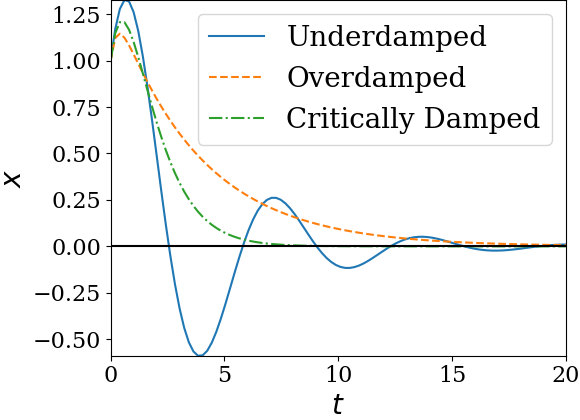
\includegraphics[scale=0.6]{phys232/Ch3-damped-oscillators-graph.png} \caption{Three cases of damping: (a) underdamping $(\omega_0>\gamma/2)$; (b) overdamping $(\omega_0<\gamma/2)$; (c) critical damping $(\omega_0=\gamma/2)$} \label{ch3:fig-damping}
\end{figure}


The motion is no longer oscillatory -- see Figure~\ref{ch3:fig-damping}b.

Recall that the solution to \eqref{ch3:eq-damping-NL} was of the form:
\[ 	x = \Re\left[ A_0 e^{-\gamma t/2} e^{j(\omega t+\alpha)} \right] \]
where
\[ \omega^2 = \omega_0^2 - \frac{\gamma^2}{4} \]
\[ \Longrightarrow \omega^2 =  -\left( \frac{\gamma^2}{4} - \omega_0^2 \right)  \]

Solving for $\omega$:
\[ \omega = \pm j\sqrt{ \frac{\gamma^2}{4}-\omega_0^2  } = \pm j\beta \]

Because of the two possibilities for $\omega$, we can write our solution more generally as%
\footnote{This is the same reasoning we used to obtain the ``more-general" solution in \eqref{ch3:eq-complex-general-sol}}:
\[ \boxed{ \therefore
x = A_1 e^{-(\gamma/2 + \beta)t} + A_2 e^{-(\gamma/2-\beta)t} 
\where \beta = \sqrt{\frac{\gamma^2}{4}-\omega_0^2} 
} \]

Note that $\beta$ is only defined when $\omega_0^2 < \gamma^2/4$.

\subsection{Critical Damping ($ \omega_0 = \gamma/2 $)}
\[ \boxed{x = (A + Bt) e^{\gamma t/2}} \]

When a force is applied to a critically damped system at rest, there will be a smooth approach to a new equilibrium position without oscillation or overshoot -- see Figure~\ref{ch3:fig-damping}c.